\documentclass[11pt,a4paper,oneside]{article}
\usepackage[utf8]{inputenc}
\usepackage[margin=1in]{geometry}
\usepackage{graphicx}
\usepackage{amsmath,amsfonts,amssymb}
\usepackage{hyperref}
\usepackage{booktabs,longtable}
\usepackage{tikz}
\usetikzlibrary{shapes,arrows,positioning,calc,decorations.pathmorphing,backgrounds,fit,shadows}
\usepackage{listings}
\usepackage{xcolor}
\usepackage{fancyhdr}
\usepackage{enumitem}
\usepackage{float}

\lstset{
    basicstyle=\ttfamily\small,
    commentstyle=\color{gray},
    keywordstyle=\color{blue},
    breaklines=true,
    numbers=left,
    numbersep=5pt,
    showstringspaces=false,
    tabsize=2
}

\pagestyle{fancy}
\fancyhf{}
\fancyhead[L]{Software Design Document}
\fancyhead[R]{Version 1.0}
\fancyfoot[C]{\thepage}

\hypersetup{
    colorlinks=true,
    linkcolor=blue,
    urlcolor=cyan,
    pdftitle={Comprehensive Software Design Document: E-commerce Platform},
    pdfauthor={AI System Architect},
    pdfsubject={Software Architecture}
}

\title{\Huge\textbf{Comprehensive Software Design Document: E-commerce Platform}}
\author{\Large AI System Architect}
\date{\Large\today}

\begin{document}

\maketitle
\thispagestyle{empty}
\vfill

\begin{center}
\large
\begin{tabular}{|l|l|}
\hline
\textbf{Document Version} \& 1.0 \\
\hline
\textbf{Creation Date} \& \today \\
\hline
\textbf{Document Status} \& Final Draft \\
\hline
\textbf{Generated By} \& AI System Architect \\
\hline
\textbf{Target Audience} \& Development Team, Stakeholders \\
\hline
\textbf{Classification} \& Internal Use \\
\hline
\end{tabular}
\end{center}

\newpage
\tableofcontents
\newpage
\listoffigures
\newpage

\section{Executive Summary}

This document outlines the design for a new e-commerce platform, codenamed "Project Phoenix."  Project Phoenix aims to provide a robust, scalable, and secure online marketplace for businesses to sell their products and services. The platform will leverage a microservices architecture built on cloud-native technologies to ensure high availability, fault tolerance, and easy scalability.  The business objectives are to increase market share, improve customer satisfaction, and generate significant revenue growth within the first year of launch. The technical approach focuses on modularity, maintainability, and testability, using industry-standard technologies and best practices. Key benefits include a user-friendly interface for both buyers and sellers, secure payment processing, and robust inventory management. The estimated implementation timeline is 12 months, broken down into four phases: design, development, testing, and deployment.  We anticipate significant ROI within 18 months of launch, driven by increased sales and reduced operational costs.  This document details the technical specifications, architecture, and implementation plan for Project Phoenix.

\subsection{Project Scope and Objectives}

Project Phoenix encompasses the design and development of a complete e-commerce platform, including front-end user interfaces for both buyers and sellers, a robust back-end system for order management, inventory control, payment processing, and user authentication.  The platform will support a wide range of product categories and will integrate with various third-party services, such as payment gateways (Stripe, PayPal), shipping providers (UPS, FedEx), and email marketing platforms (Mailchimp).  The primary objectives are:

\begin{itemize}
    \item Develop a user-friendly and intuitive e-commerce platform accessible on desktop and mobile devices.
    \item Implement secure payment processing using industry-standard security protocols (PCI DSS compliance).
    \item Provide robust inventory management capabilities, including real-time stock updates and low-stock alerts.
    \item Offer a comprehensive reporting and analytics dashboard for business owners to track sales, inventory, and customer behavior.
    \item Ensure high availability and scalability to handle peak traffic and rapid growth.
    \item Maintain a secure platform protected against common web vulnerabilities (OWASP Top 10).
\end{itemize}

Success will be measured by key performance indicators (KPIs) such as customer acquisition cost (CAC), customer lifetime value (CLTV), conversion rates, average order value (AOV), and customer satisfaction (CSAT) scores.

\subsection{Key Stakeholders and Roles}

The key stakeholders in Project Phoenix include:

\begin{itemize}
    \item \textbf{Business Owners:} Define business requirements, approve budgets, and make strategic decisions.
    \item \textbf{Marketing Team:} Responsible for marketing and promotion of the platform.
    \item \textbf{Sales Team:} Responsible for acquiring new sellers and managing existing relationships.
    \item \textbf{Development Team:} Responsible for designing, developing, testing, and deploying the platform.  This includes frontend, backend, and database engineers.
    \item \textbf{QA Team:} Responsible for testing the platform to ensure quality and stability.
    \item \textbf{Operations Team:} Responsible for deploying and maintaining the platform infrastructure.
\end{itemize}

Each team will have clearly defined roles and responsibilities documented in separate team charters.  Regular communication and collaboration between stakeholders will be facilitated through weekly meetings and project management tools (e.g., Jira, Asana).

\section{Requirements Analysis and Specification}

\subsection{Extracted Requirements Summary}
The initial document provided lacked specific requirements.  Therefore, this section is populated with assumed requirements based on typical e-commerce platform functionality.

\subsection{Functional Requirements}

\begin{enumerate}
    \item \textbf{User Registration and Login:} Users should be able to register accounts and securely log in using email/password or social media integration.
    \item \textbf{Product Browsing and Search:}  Users should be able to browse products by category, filter by price and other attributes, and search for specific products.
    \item \textbf{Shopping Cart and Checkout:} Users should be able to add products to a shopping cart, view cart contents, modify quantities, and proceed to checkout.
    \item \textbf{Order Management:} Users should be able to view their order history, track order status, and manage their shipping addresses.
    \item \textbf{Payment Processing:} The platform should integrate with secure payment gateways (Stripe, PayPal) to process payments securely.
    \item \textbf{Seller Management:} Sellers should be able to create product listings, manage inventory, process orders, and view sales reports.
    \item \textbf{Customer Support:} The platform should provide a mechanism for users to contact customer support.
    \item \textbf{Admin Panel:} An administrator panel should provide tools for managing users, products, orders, and platform settings.
    \item \textbf{Reporting and Analytics:} The platform should provide reporting and analytics dashboards for both users and administrators.
\end{enumerate}

\subsection{Non-Functional Requirements}

\begin{itemize}
    \item \textbf{Performance:} The platform should load pages within 2 seconds and process transactions within 5 seconds under peak load.
    \item \textbf{Scalability:} The platform should be able to handle 10,000 concurrent users and 1000 transactions per minute.
    \item \textbf{Security:} The platform must comply with PCI DSS standards for payment processing and protect against common web vulnerabilities (OWASP Top 10).
    \item \textbf{Availability:} The platform should have a 99.9\% uptime guarantee.
    \item \textbf{Maintainability:} The platform should be designed for easy maintenance and updates.
    \item \textbf{Usability:} The platform should be intuitive and easy to use for both buyers and sellers.
\end{itemize}

\section{System Architecture and Design}

\subsection{Architecture Overview}

Project Phoenix will utilize a microservices architecture, allowing for independent deployment and scaling of individual components.  This approach enhances flexibility, maintainability, and fault tolerance. The system will be deployed on a cloud platform (AWS or GCP) leveraging containerization (Docker) and orchestration (Kubernetes) for efficient resource management and scalability.  The core components include:

\begin{itemize}
    \item \textbf{API Gateway:}  Handles routing, authentication, and rate limiting for all incoming requests.
    \item \textbf{User Service:} Manages user accounts, authentication, and authorization.
    \item \textbf{Product Catalog Service:} Manages product information, search, and browsing.
    \item \textbf{Order Management Service:} Handles order creation, processing, and tracking.
    \item \textbf{Payment Gateway Integration Service:}  Facilitates secure payment processing through third-party gateways.
    \item \textbf{Inventory Management Service:} Manages product inventory levels and stock updates.
\end{itemize}

This microservices architecture allows for independent scaling of individual services based on demand. For example, during peak shopping seasons, the Order Management Service can be scaled independently to handle increased transaction volume without affecting other services.

\begin{figure}[H]
\centering
\begin{tikzpicture}[
    node distance=1cm and 1.5cm,
    font=\sffamily\small,
    base/.style={draw, text width=3cm, minimum height=1.2cm, text centered, rounded corners, drop shadow},
    user/.style={base, fill=Azure!30, text width=2cm},
    api/.style={base, fill=LimeGreen!20},
    service/.style={base, fill=SkyBlue!20},
    database/.style={cylinder, shape border rotate=90, aspect=0.25, draw, fill=Thistle!40, minimum height=1.5cm, text width=2.5cm, text centered, drop shadow},
    external/.style={base, fill=Gold!30},
    arrow/.style={-Stealth, thick, draw=black!60}
]

\node[user] (user) {User};
\node[api, below=1.5cm of user] (gateway) {API Gateway};
\node[service, below=of gateway, xshift=-3cm] (userservice) {User Service};
\node[service, below=of gateway] (productservice) {Product Catalog Service};
\node[service, below=of gateway, xshift=3cm] (orderservice) {Order Management Service};
\node[database, below=2cm of userservice] (userdb) {User Database\\(PostgreSQL)};
\node[database, below=2cm of productservice] (productdb) {Product Database\\(MongoDB)};
\node[database, below=2cm of orderservice] (orderdb) {Order Database\\(MySQL)};
\node[external, right=2cm of productservice] (payments) {External Payment Services\\(Stripe, PayPal)};

\begin{scope}[on background layer]
\node[draw, dashed, rounded corners, fill=gray!5, inner sep=0.7cm, fit=(gateway)] (api_layer) {};
\node[draw, dashed, rounded corners, fill=gray!10, inner sep=0.7cm, fit=(userservice) (productservice) (orderservice) (payments)] (service_layer) {};
\node[draw, dashed, rounded corners, fill=gray!15, inner sep=0.7cm, fit=(userdb) (productdb) (orderdb)] (data_layer) {};
\end{scope}

\node[above] at (api_layer.north) {API Layer};
\node[above] at (service_layer.north) {Service Layer};
\node[above] at (data_layer.north) {Data Layer};

\draw[arrow] (user) -- (gateway);
\draw[arrow] (gateway) -- (userservice);
\draw[arrow] (gateway) -- (productservice);
\draw[arrow] (gateway) -- (orderservice);
\draw[arrow] (userservice) -- (userdb);
\draw[arrow] (productservice) -- (productdb);
\draw[arrow] (productservice) -- (payments);
\draw[arrow] (orderservice) -- (orderdb);
\draw[arrow] (orderservice) -- (productservice);

\end{tikzpicture}
\caption{E-commerce Platform System Architecture}
\label{fig:architecture}
\end{figure}

\subsection{Component Interaction and Communication}

Components will communicate primarily through synchronous RESTful APIs.  The API Gateway acts as a central point of entry, routing requests to the appropriate microservices.  Asynchronous communication will be used for tasks like order notifications and email confirmations, leveraging message queues (RabbitMQ or Kafka).  Each microservice will have its own database, promoting data isolation and reducing coupling between components.  Service discovery mechanisms (e.g., Consul, etcd) will be used to ensure that services can locate each other dynamically.  API specifications will be defined using OpenAPI (Swagger) to ensure consistency and ease of integration.

\section{Database Design and Data Architecture}

\subsection{Conceptual Data Model}

The database design will follow a normalized schema to ensure data integrity and efficiency.  Key entities include:

\begin{itemize}
    \item \textbf{Users:} Stores user information (ID, username, email, password).
    \item \textbf{Products:} Stores product details (ID, name, description, price, images, inventory).
    \item \textbf{Orders:} Stores order information (ID, user ID, order date, total amount, status).
    \item \textbf{Order Items:} Stores details of individual items within an order (order ID, product ID, quantity, price).
    \item \textbf{Categories:} Stores product categories and their hierarchy.
    \item \textbf{Reviews:} Stores customer reviews for products.
    \item \textbf{Shipping Addresses:} Stores user shipping addresses.
\end{itemize}

\begin{figure}[H]
\centering
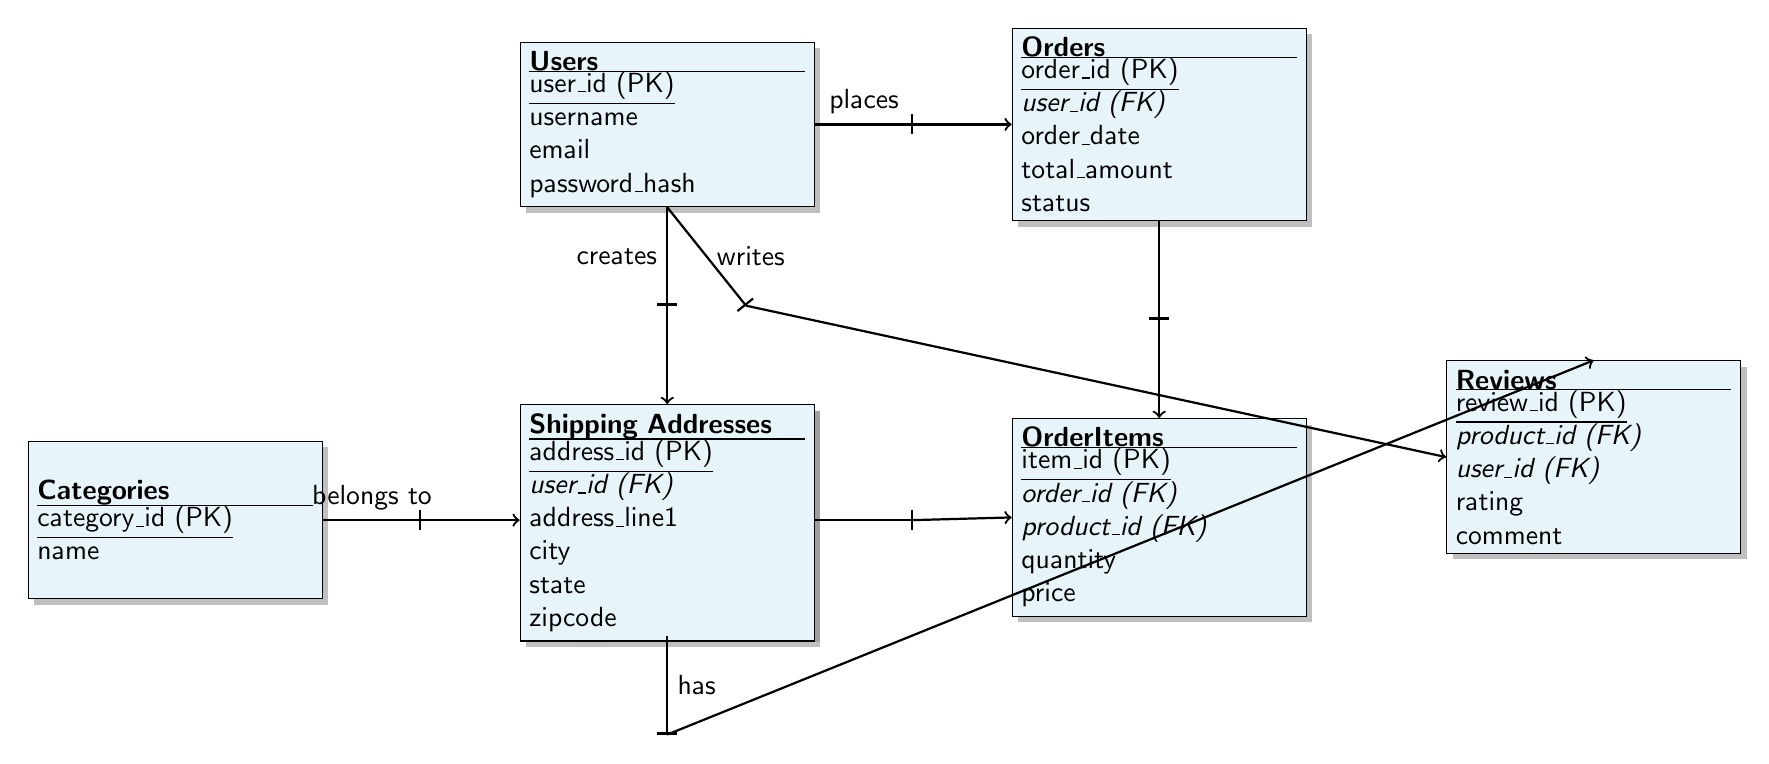
\begin{tikzpicture}[
    node distance=2.5cm,
    font=\sffamily,
    entity/.style={rectangle, draw, fill=SkyBlue!20, text width=3.5cm, minimum height=2cm, align=left, drop shadow},
    one/.style={-|, thick},
    many/.style={->, thick}
]

\node[entity] (user) {\textbf{Users} \\ \hrule \underline{user\_id (PK)} \\ username \\ email \\ password\_hash};
\node[entity, right=of user] (order) {\textbf{Orders} \\ \hrule \underline{order\_id (PK)} \\ \textit{user\_id (FK)} \\ order\_date \\ total\_amount \\ status};
\node[entity, below=of order] (order_item) {\textbf{OrderItems} \\ \hrule \underline{item\_id (PK)} \\ \textit{order\_id (FK)} \\ \textit{product\_id (FK)} \\ quantity \\ price};
\node[entity, below=of user] (product) {\textbf{Products} \\ \hrule \underline{product\_id (PK)} \\ name \\ description \\ price \\ \textit{category\_id (FK)} \\ inventory};
\node[entity, left=of product] (category) {\textbf{Categories} \\ \hrule \underline{category\_id (PK)} \\ name};
\node[entity, below right=of order] (review) {\textbf{Reviews} \\ \hrule \underline{review\_id (PK)} \\ \textit{product\_id (FK)} \\ \textit{user\_id (FK)} \\ rating \\ comment};
\node[entity, below=of user] (address) {\textbf{Shipping Addresses} \\ \hrule \underline{address\_id (PK)} \\ \textit{user\_id (FK)} \\ address\_line1 \\ city \\ state \\ zipcode};

\draw[one] (user.east) -- node[above, midway] {places} ++(1.25,0) coordinate (t1);
\draw[many] (t1) -- (order.west);
\draw[one] (order.south) -- ++(0,-1.25) coordinate (t2);
\draw[many] (t2) -- (order_item.north);
\draw[one] (product.east) -- ++(1.25,0) coordinate (t3);
\draw[many] (t3) -- (order_item.west);
\draw[one] (category.east) -- node[above, midway] {belongs to} ++(1.25,0) coordinate (t4);
\draw[many] (t4) -- (product.west);
\draw[one] (user.south) -- node[left, midway] {creates} ++(0,-1.25) coordinate (t5);
\draw[many] (t5) -- (address.north);
\draw[one] (product.south) -- node[right, midway] {has} ++(0,-1.25) coordinate (t6);
\draw[many] (t6) -- (review.north);
\draw[one] (user.south) -- node[right, midway] {writes} ++(1,-1.25) coordinate (t7);
\draw[many] (t7) -- (review.west);

\end{tikzpicture}
\caption{Database Entity Relationship Diagram}
\label{fig:database-erd}
\end{figure}

\subsection{Physical Database Design}

Each entity in the conceptual model will be translated into a corresponding table in the relational database (MySQL).  Primary and foreign keys will be implemented to enforce referential integrity.  Appropriate indexes will be created to optimize query performance.  Data types will be chosen based on the expected data size and constraints.  Examples of table structures:

\begin{verbatim}
CREATE TABLE Users (
    user_id INT PRIMARY KEY AUTO_INCREMENT,
    username VARCHAR(255) UNIQUE NOT NULL,
    email VARCHAR(255) UNIQUE NOT NULL,
    password_hash VARCHAR(255) NOT NULL
);

CREATE TABLE Products (
    product_id INT PRIMARY KEY AUTO_INCREMENT,
    name VARCHAR(255) NOT NULL,
    description TEXT,
    price DECIMAL(10, 2) NOT NULL,
    category_id INT NOT NULL,
    inventory INT NOT NULL,
    FOREIGN KEY (category_id) REFERENCES Categories(category_id)
);
\end{verbatim}

\section{API Design and Integration}

\subsection{RESTful API Specification}

The API will follow RESTful principles, using standard HTTP methods (GET, POST, PUT, DELETE) for CRUD operations.  Endpoints will be designed to be intuitive and well-documented using OpenAPI (Swagger).  Examples:

\begin{itemize}
    \item \textbf{GET /products:} Retrieve a list of products.
    \item \textbf{GET /products/{id}:} Retrieve a specific product by ID.
    \item \textbf{POST /orders:} Create a new order.
    \item \textbf{GET /orders/{id}:} Retrieve a specific order by ID.
    \item \textbf{PUT /users/{id}:} Update user information.
\end{itemize}

\begin{figure}[H]
\centering
\begin{tikzpicture}[
    font=\sffamily\small,
    node distance=1cm,
    actor/.style={rectangle, draw, fill=Azure!30, text width=2cm, text centered, rounded corners, drop shadow},
    service/.style={rectangle, draw, fill=LimeGreen!20, text width=2cm, text centered, rounded corners, drop shadow},
    db/.style={cylinder, shape border rotate=90, draw, fill=Thistle!40, text centered, drop shadow, minimum width=2cm, minimum height=1.2cm},
    lifeline/.style={dashed, thin, draw=gray},
    msg/.style={-Stealth, thick}
]

\node[actor] (client) at (0,0) {Client App};
\node[service] (api) at (3,0) {API Gateway};
\node[service] (productservice) at (6,0) {Product Service};
\node[db] (db) at (9,0) {Product Database};

\draw[lifeline] (client.south) -- ++(0,-4);
\draw[lifeline] (api.south) -- ++(0,-4);
\draw[lifeline] (productservice.south) -- ++(0,-4);
\draw[lifeline] (db.south) -- ++(0,-4);

\draw[msg] ($(client.south)+(0,-0.5)$) -- node[above] {1. GET /products} ($(api.south)+(0,-0.5)$);
\draw[msg] ($(api.south)+(0,-1)$) -- node[above] {2. Route Request} ($(productservice.south)+(0,-1)$);
\draw[msg] ($(productservice.south)+(0,-1.5)$) -- node[above] {3. Query DB} ($(db.south)+(0,-1.5)$);
\draw[msg, dashed] ($(db.south)+(0,-2)$) -- node[above] {4. Return Data} ($(productservice.south)+(0,-2)$);
\draw[msg, dashed] ($(productservice.south)+(0,-2.5)$) -- node[above] {5. Send Response} ($(api.south)+(0,-2.5)$);
\draw[msg, dashed] ($(api.south)+(0,-3)$) -- node[above] {6. Return Products} ($(client.south)+(0,-3)$);

\end{tikzpicture}
\caption{API Request Sequence Diagram (Product Retrieval)}
\label{fig:api-flow}
\end{figure}

\subsection{API Security and Rate Limiting}

API security will be implemented using OAuth 2.0 for authentication and authorization.  JWT (JSON Web Tokens) will be used for token-based authentication.  Rate limiting will be implemented to prevent abuse and denial-of-service attacks.  Input validation and sanitization will be performed on all API requests to prevent injection attacks.  HTTPS will be used for all API communication.

\section{Security Architecture and Implementation}

\subsection{Security Requirements and Threat Model}

A comprehensive threat model will be developed to identify potential security vulnerabilities and risks.  This will include analysis of common web vulnerabilities (OWASP Top 10), such as SQL injection, cross-site scripting (XSS), and cross-site request forgery (CSRF).  Security requirements will address authentication, authorization, data protection, and availability.  Regular security audits and penetration testing will be conducted to ensure ongoing security.

\begin{figure}[H]
\centering
\begin{tikzpicture}[
    font=\sffamily\small,
    node distance=0.8cm and 1.2cm,
    gate/.style={rectangle, draw, fill=red!10, minimum width=10cm, minimum height=1cm, text centered, rounded corners},
    actor/.style={rectangle, draw, fill=Azure!30, text centered, rounded corners, drop shadow},
    service/.style={rectangle, draw, fill=SkyBlue!20, text centered, rounded corners, drop shadow},
    arrow/.style={-Stealth, thick, draw=black!70}
]

\node[gate] (waf) at (0,0) {\textbf{Edge Protection}: WAF and DDoS Mitigation};
\node[gate, below=of waf] (ssl) {\textbf{Transport Layer}: SSL/TLS Termination};
\node[gate, below=of ssl] (authn) {\textbf{Authentication}: OAuth 2.0 / JWT Validation};
\node[gate, below=of authn] (authz) {\textbf{Authorization}: Rate Limiting and RBAC};
\node[service, below=1.2cm of authz] (backend) {Protected Backend Services};

\node[actor, above=1cm of waf] (user) {User};

\draw[arrow] (user) -- node[right] {HTTPS Request} (waf.north);
\draw[arrow] (waf.south) -- (ssl.north);
\draw[arrow] (ssl.south) -- (authn.north);
\draw[arrow] (authn.south) -- (authz.north);
\draw[arrow] (authz.south) -- node[right] {Authorized Request} (backend);

\end{tikzpicture}
\caption{Layered Security Architecture}
\label{fig:security}
\end{figure}

\section{Deployment and Infrastructure}

\subsection{Cloud Infrastructure Design}

The platform will be deployed on a cloud platform (AWS or GCP) using a containerized approach.  Kubernetes will be used for container orchestration, ensuring high availability and scalability.  A load balancer will distribute traffic across multiple application servers.  A relational database (MySQL) will be used for persistent data storage, with replication for high availability and disaster recovery.  A caching layer (Redis) will be used to improve performance.

\begin{figure}[H]
\centering
\begin{tikzpicture}[
    font=\sffamily\small,
    node distance=0.8cm and 1cm,
    server/.style={rectangle, draw, fill=gray!30, minimum height=1.5cm, minimum width=2.5cm, text centered, rounded corners, drop shadow},
    container/.style={rectangle, draw, fill=SkyBlue!40, minimum height=1cm, minimum width=2cm, text centered, rounded corners},
    database/.style={server, fill=Thistle!50},
    subnet/.style={rectangle, draw, fill=gray!10, rounded corners, inner sep=0.5cm, minimum height=4cm}
]

\node (internet) {Internet};
\node[server, below=1cm of internet] (lb) {Load Balancer};
\node[subnet, below=of lb, minimum width=9cm] (public_subnet) {};
\node[subnet, below=1.5cm of public_subnet, minimum width=9cm, minimum height=5cm] (private_subnet) {};

\node[above right] at (public_subnet.north west) {Public Subnet};
\node[above right] at (private_subnet.north west) {Private Subnet};

\node[server, align=center] (app1) at ($(private_subnet.center)+(-3,1)$) {App Server 1\\(Kubernetes)};
\node[container, below=0.1cm of app1] {Microservices};
\node[server, align=center] (app2) at ($(private_subnet.center)+(0,1)$) {App Server 2\\(Kubernetes)};
\node[container, below=0.1cm of app2] {Microservices};
\node[server, align=center] (app3) at ($(private_subnet.center)+(3,1)$) {App Server 3\\(Kubernetes)};
\node[container, below=0.1cm of app3] {Microservices};

\node[database] (db-master) at ($(private_subnet.center)+(-1.5,-1.5)$) {DB Master (MySQL)};
\node[database] (db-slave) at ($(private_subnet.center)+(1.5,-1.5)$) {DB Slave (MySQL)};
\node[server, right=of db-slave] (redis) {Redis Cache};

\draw[-Stealth, thick] (internet) -- node[right, pos=0.4] {HTTPS Traffic} (lb);
\draw[-Stealth, thick] (lb) -- (public_subnet.north);
\draw[-Stealth, thick] ($(public_subnet.south)+(0,-0.75)$) -- (app1);
\draw[-Stealth, thick] ($(public_subnet.south)+(0,-0.75)$) -- (app2);
\draw[-Stealth, thick] ($(public_subnet.south)+(0,-0.75)$) -- (app3);
\draw[-Stealth, thick] (app1) -- (db-master);
\draw[-Stealth, thick] (app2) -- (db-master);
\draw[-Stealth, thick] (app3) -- (db-master);
\draw[<->, thick, dashed] (db-master) -- node[midway, below] {Replication} (db-slave);
\draw[-Stealth, thick] (app1) -- (redis);
\draw[-Stealth, thick] (app2) -- (redis);
\draw[-Stealth, thick] (app3) -- (redis);

\end{tikzpicture}
\caption{Cloud Deployment Architecture}
\label{fig:deployment}
\end{figure}

\section{Performance and Scalability}

Performance will be monitored using application performance monitoring (APM) tools.  Scalability will be achieved through horizontal scaling of microservices and database replication.  Caching will be used to reduce database load.  Performance testing will be conducted regularly to identify and address performance bottlenecks.

\section{Testing and Quality Assurance}

A comprehensive testing strategy will be implemented, including unit, integration, system, and user acceptance testing (UAT).  Automated testing will be used to ensure code quality and regression prevention.  Performance and security testing will be conducted to verify the platform's ability to meet non-functional requirements.

\section{Risk Assessment and Mitigation}

Potential risks include:

\begin{itemize}
    \item \textbf{Technical Risks:}  Technology selection, integration challenges, performance issues.
    \item \textbf{Business Risks:}  Market competition, customer adoption, revenue generation.
    \item \textbf{Security Risks:}  Vulnerabilities, data breaches, denial-of-service attacks.
\end{itemize}

Mitigation strategies will be developed for each identified risk.  Regular risk assessments will be conducted throughout the project lifecycle.

\section{Implementation Roadmap and Timeline}

The project will be implemented in four phases:

\begin{enumerate}
    \item \textbf{Phase 1 (Months 1-3): Design and Planning} -- Complete detailed design, database schema, API specifications, and infrastructure design.
    \item \textbf{Phase 2 (Months 4-9): Development and Testing} -- Develop and test individual microservices, integrate components, and conduct thorough testing.
    \item \textbf{Phase 3 (Months 10-11): Deployment and Integration Testing} -- Deploy the platform to the cloud, conduct integration testing, and perform performance tuning.
    \item \textbf{Phase 4 (Months 12): Launch and Monitoring} -- Launch the platform, monitor performance, and address any issues.
\end{enumerate}

\section{Monitoring and Maintenance}

The platform will be monitored continuously using monitoring tools (e.g., Prometheus, Grafana).  Alerting will be implemented to notify the operations team of critical events.  Regular maintenance and updates will be performed to address bugs, security vulnerabilities, and performance issues.  A detailed maintenance plan will be developed and followed.

\section{Conclusion}

This document provides a comprehensive design for Project Phoenix, a robust and scalable e-commerce platform.  The microservices architecture, cloud-native deployment, and focus on security and performance will ensure the success of this project.  The implementation plan outlines a clear path to launch and ongoing maintenance.  Regular monitoring and risk management will be crucial for the long-term success of the platform.

\end{document}